
\section{Conversion de decimal a binario con signo}

\subsection{Definicion de la solución}

El problema planteado consiste en obtener el equivalente binario de un número decimal con signo. Se debe respetar la regla de conversión de complemento a dos para los números negativos, con el objetivo de diseñar un algoritmo capaz de tomar cualquier número decimal como entrada y devolver su representación binaria correspondiente.\cite{Decimal a  binario con signo}
\subsection{Descripción del problema}
Dado un numero decimal entero positivo o negativo regresar su equivalente en binario.

\subsection{Diseño de la solucion}
Para diseñar una solución viable al progreso del algoritmo, necesitaremos establcer los siguinetes pasos:

\begin{enumerate}

\item Definir el número decimal para después convertir a binario.

\item Invertir los \texttt{bits}.

\item Sumar 1 al \texttt{bit} menos significativo. Así obtendremos el complemento a dos.
\end{enumerate}

 \begin {figure}[h!]
\centerline{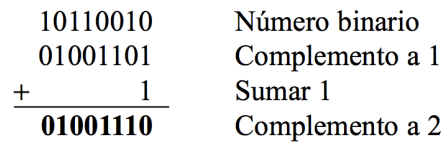
\includegraphics[width = 5cm]{imagen/ejemploa2.png}}
\caption{Procedimineto del complemento a dos.}
\label{fig}
\end {figure}

\subsection{Desarrollo de la solución}
Se presentará el algoritmo, desarrollado en el lenguaje de programación JAVA.

\lstset{
  language=Java,
  basicstyle=\ttfamily,
  keywordstyle=\bfseries,
  commentstyle=\itshape,
  showstringspaces=false,
  columns=flexible,
  frame=single,
  numbers=left,
  numberstyle=\tiny,
  breaklines=true,
  captionpos=b
}

\begin{javaCode}


import java.util.Scanner;
public class Ejercicio4 {

  
    public static void main(String[] args) {
        //entrada
             Scanner entrada = new Scanner(System.in);

        // Solicitar al usuario que ingrese un número decimal
        System.out.print("Ingrese un número decimal: ");
        int numeroDecimal = entrada.nextInt();

        // Verificar si el número es negativo
        boolean esNegativo = false;
        if (numeroDecimal < 0) {
            esNegativo = true;
            numeroDecimal = Math.abs(numeroDecimal);
        }

        // Inicializar una cadena para almacenar el número binario
        String numeroBinario = "";

        // Manejar el caso especial cuando el número decimal es 0
        if (numeroDecimal == 0) {
            numeroBinario = "0";
        } else {
            // Convertir el número decimal a binario
            while (numeroDecimal > 0) {
                int residuo = numeroDecimal % 2; // Obtener el residuo de la división por 2
                numeroBinario = residuo + numeroBinario; // Agregar el residuo al inicio de la cadena binaria
                numeroDecimal = numeroDecimal / 2; // Dividir el número decimal por 2
            }

            // Calcular el complemento a dos si el número es negativo
            if (esNegativo) {
                StringBuilder complementoBuilder = new StringBuilder();
                boolean encontradoPrimerUno = false;

                // Invertir los bits
                for (int i = numeroBinario.length() - 1; i >= 0; i--) {
                    char bit = numeroBinario.charAt(i);
                    if (!encontradoPrimerUno) {
                 
                        if (bit == '1') {
                            encontradoPrimerUno = true;
                        }
                        complementoBuilder.insert(0, bit);
                    } else {
                        // Invertir los bits restantes
                        if (bit == '0') {
                            complementoBuilder.insert(0, '1');
                        } else {
                            complementoBuilder.insert(0, '0');
                        }
                    }
                }

                numeroBinario = complementoBuilder.toString();
            }
        }

        // Agregar signo negativo si corresponde
        if (esNegativo) {
            numeroBinario = "" + numeroBinario;
        }

        // Imprimir el número binario resultante
        System.out.println("El número binario equivalente es: " + numeroBinario);
    }
}
    \end{javaCode}
\\
\subsection{Depuración y pruebas}

La siguiente tabla muestra los resultados del programa en JAVA, que constituyen el resultado final.

\begin{tabular}{|c|c|c|}
  \hline
  \textbf{No.de corridas} & \textbf{No.Decimal} & \textbf{Complemento a 2} \\
  \hline
  1 & -28 & 00100 \\
  \hline
  2 & 222 & 11011110 \\
  \hline
  3 & -1480 & 01000111000 \\
  \hline
  4 & 10 & 1010  \\ 
  \hline
\end{tabular}
\caption{Tabla de corridas.}









